\documentclass[11pt]{article}
\usepackage[T1]{fontenc}\usepackage[utf8]{inputenc}\usepackage{lmodern}\usepackage{amsmath,amssymb}
\usepackage[margin=1in]{geometry}\usepackage{longtable,booktabs}\usepackage{graphicx}\usepackage[hidelinks]{hyperref}
\title{Blueprint: Coefficient choice in Galois-ring lifts of APN permutations}
\author{Hiroki Fukui}
\date{Version 2.0.0, 27 October 2026}
\begin{document}\maketitle
\section*{Purpose}
This blueprint maps every result of the paper \emph{Coefficient choice in Galois-ring lifts of APN permutations: sharp
unit-direction spectra and one-term optimal lifts} to the Lean~4 declarations that formalize it, states what remains
on paper, and names the finite computations that cross-check it. Numbers refer to the paper (\texttt{paper/manuscript.pdf}).
The Lean development is in \texttt{supplement/lean} (Lean 4.31.0-rc1, Mathlib \texttt{d568c8c}): 55 modules, the root
\texttt{Apn2R03.lean} and \texttt{Audit.lean}. \texttt{Audit.lean} prints the axioms of 150 declarations; in the author's
clean build every one depends only on \texttt{propext}, \texttt{Classical.choice} and \texttt{Quot.sound}, and no
declaration uses \texttt{sorry}. This blueprint was generated by \texttt{blueprint/gen\_blueprint.py}, which checks that
every declaration named below is audited in \texttt{Audit.lean} and defined in exactly one module.

\paragraph{Settings.} Most results are proved for an abstract finite ring $R$ with a surjection onto a finite field $K$
whose kernel is $2R$, with $2^k=0$ and $2$-torsion $2^{k-1}R$; the declarations \texttt{grs}, \texttt{grs\_card} and
\texttt{exists\_GR\_poly} show that $\mathrm{GR}(2^k,m)$ satisfies these axioms, and the declarations ending in
\texttt{\_GR} state results on the concrete ring. Difference counts are cardinalities of actual finite solution sets.

\paragraph{Status.} 22 nodes; ``formalized'' means that every mathematical claim of the item is a Lean theorem;
otherwise the paper-only parts are listed.

\begin{longtable}{p{0.13\textwidth}p{0.47\textwidth}p{0.32\textwidth}}\toprule Paper & Item & Status\\\midrule\endhead
Lemma 4.1 & Lift invariants A\_F and E\_F are well defined; their control & formalized\\
Lemma 3.2 & Hypothesis (H) gives the abstract hypotheses used in Lean & formalized\\
Section 3 & Galois rings satisfy the abstract axioms used in Lean & formalized\\
Theorem B & Minimax over all lifts & formalized\\
Theorem C & All minimizers & formalized\\
Theorem D & Exceptional spectra and certification modulo 8 & formalized\\
Corollary E & Optimality across levels (and Theorem 6.3, Corollary 6.4) & formalized\\
Theorem F & Penultimate layer, middle layer at $k=3$, and the trade-off & formalized\\
Theorem 8.4 & Intermediate layers (Theorem 8.4) and Corollary 8.5 & formalized\\
Proposition 7.1 & The residue $P_{m,r}$ is an APN permutation & formalized\\
Theorem A & A one-term optimal lift of $P_{m,r}$ & core formalized; parts on paper\\
Corollary 7.5 & The natural lift at $k=3$ & formalized\\
Proposition 9.1 & Valuation preservation & formalized\\
Proposition 9.3 & Markov property and product bound for characteristics (Corollary G (a)) & formalized\\
Proposition 9.4 & Characteristics in every 2-adic layer (Corollary G (b)) & formalized\\
Proposition 9.5 & Two-round differentials for every lift (Corollary G (c), first part) & core formalized; parts on paper\\
Proposition 9.6 & Layerwise two-round differential bounds without a support factor (Corollary G (c), second part) & core formalized; parts on paper\\
Proposition 9.7 & Fixed keys (Corollary G (d)) & formalized\\
Proposition 9.8 & Residue partition & core formalized; parts on paper\\
Theorem 10.1 & Representatives with $\mu=0$ and $Z=\emptyset$ for every odd m & core formalized; parts on paper\\
Theorem 10.2 & A sparse family (at most 16 monomials) & core formalized; parts on paper\\
Proposition 10.3 & Low-cost optimal lifts by one coefficient digit & formalized for the family $P_{m,r}$; general case on paper\\
\bottomrule\end{longtable}
\subsection*{Lemma 4.1 (p.~7): Lift invariants A\_F and E\_F are well defined; their control}
\textbf{Status:} formalized.\par
\textbf{Lean:}\begin{itemize}\setlength\itemsep{0pt}
\item \texttt{APN2.GRS.A\_spec} \hfill (\texttt{Apn2R03/Invariants.lean})
\item \texttt{APN2.GRS.E\_spec} \hfill (\texttt{Apn2R03/Invariants.lean})
\item \texttt{APN2.GRS.E\_transl} \hfill (\texttt{Apn2R03/Invariants.lean})
\item \texttt{APN2.GRS.A\_prescribe} \hfill (\texttt{Apn2R03/Control.lean})
\item \texttt{APN2.GRS.E\_prescribe} \hfill (\texttt{Apn2R03/Control.lean})
\item \texttt{APN2.GRS.A\_control} \hfill (\texttt{Apn2R03/Control.lean})
\item \texttt{APN2.GRS.E\_control} \hfill (\texttt{Apn2R03/Control.lean})
\end{itemize}
\subsection*{Lemma 3.2 (p.~6): Hypothesis (H) gives the abstract hypotheses used in Lean}
\textbf{Status:} formalized.\par
\textbf{Lean:}\begin{itemize}\setlength\itemsep{0pt}
\item \texttt{APN2.GRS.hyp\_of\_H} \hfill (\texttt{Apn2R03/HypFromH.lean})
\end{itemize}
\subsection*{Section 3 (p.~6): Galois rings satisfy the abstract axioms used in Lean}
\textbf{Status:} formalized.\par
\textbf{Lean:}\begin{itemize}\setlength\itemsep{0pt}
\item \texttt{APN2.grs} \hfill (\texttt{Apn2R03/GRInst.lean})
\item \texttt{APN2.grs\_card} \hfill (\texttt{Apn2R03/GRInst.lean})
\item \texttt{APN2.exists\_GR\_poly} \hfill (\texttt{Apn2R03/MainGR.lean})
\item \texttt{APN2.zmod8} \hfill (\texttt{Apn2R03/Basic.lean})
\end{itemize}
\subsection*{Theorem B (p.~4): Minimax over all lifts}
\textbf{Status:} formalized.\par
\textbf{Lean:}\begin{itemize}\setlength\itemsep{0pt}
\item \texttt{APN2.GRS.minimax\_k3\_attain} \hfill (\texttt{Apn2R03/MainK3.lean})
\item \texttt{APN2.GRS.minimax\_k4\_attain} \hfill (\texttt{Apn2R03/MainK4.lean})
\item \texttt{APN2.GRS.minimax\_k3\_lower} \hfill (\texttt{Apn2R03/MainK3.lean})
\item \texttt{APN2.GRS.minimax\_k4\_lower} \hfill (\texttt{Apn2R03/MainK4.lean})
\end{itemize}
\textbf{Computational cross-check:} validate\_v3 at $m=5$ (32 records: 27 MATCH, 5 BOUND\_ONLY).\par
\textbf{Uses:} Lemma 4.1, Lemma 3.2.\par
\subsection*{Theorem C (p.~5): All minimizers}
\textbf{Status:} formalized.\par
\textbf{Lean:}\begin{itemize}\setlength\itemsep{0pt}
\item \texttt{APN2.GRS.minimizers\_k3} \hfill (\texttt{Apn2R03/MainK3.lean})
\item \texttt{APN2.GRS.minimizers\_k4} \hfill (\texttt{Apn2R03/MainK4.lean})
\end{itemize}
\textbf{Computational cross-check:} validate\_v3.\par
\textbf{Uses:} Theorem B.\par
\subsection*{Theorem D (p.~5): Exceptional spectra and certification modulo 8}
\textbf{Status:} formalized.\par
\textbf{Lean:}\begin{itemize}\setlength\itemsep{0pt}
\item \texttt{APN2.GRS.spectrum\_mu0} \hfill (\texttt{Apn2R03/Spectrum3.lean})
\item \texttt{APN2.GRS.spectrum\_mu} \hfill (\texttt{Apn2R03/Spectrum2.lean})
\item \texttt{APN2.GRS.spectrum\_k3} \hfill (\texttt{Apn2R03/Spectrum4.lean})
\item \texttt{APN2.GRS.delta\_stable\_mod8} \hfill (\texttt{Apn2R03/StabilityLit.lean})
\item \texttt{APN2.delta\_stable\_mod8\_GR} \hfill (\texttt{Apn2R03/StabilityLit.lean})
\end{itemize}
\textbf{Computational cross-check:} validate\_v3, e\_tests.\par
\textbf{Uses:} Lemma 4.1.\par
\subsection*{Corollary E (p.~5): Optimality across levels (and Theorem 6.3, Corollary 6.4)}
\textbf{Status:} formalized.\par
\textbf{Lean:}\begin{itemize}\setlength\itemsep{0pt}
\item \texttt{APN2.GRS.cross\_level\_stay} \hfill (\texttt{Apn2R03/CrossLevel.lean})
\item \texttt{APN2.GRS.cross\_level\_exists} \hfill (\texttt{Apn2R03/CrossLevel.lean})
\item \texttt{APN2.cross\_level\_stay\_GR} \hfill (\texttt{Apn2R03/GRCompat.lean})
\item \texttt{APN2.cross\_level\_exists\_GR} \hfill (\texttt{Apn2R03/GRCompat.lean})
\item \texttt{APN2.GRS.coherent\_family} \hfill (\texttt{Apn2R03/Coherent.lean})
\item \texttt{APN2.coherent\_family\_GR} \hfill (\texttt{Apn2R03/GRTower.lean})
\item \texttt{APN2.towerGR} \hfill (\texttt{Apn2R03/GRTower.lean})
\end{itemize}
\textbf{Computational cross-check:} tests/test\_cross\_level.py.\par
\textbf{Uses:} Theorem C, Theorem D.\par
\subsection*{Theorem F (p.~5): Penultimate layer, middle layer at $k=3$, and the trade-off}
\textbf{Status:} formalized.\par
\textbf{Lean:}\begin{itemize}\setlength\itemsep{0pt}
\item \texttt{APN2.GRS.penultimate} \hfill (\texttt{Apn2R03/Layers.lean})
\item \texttt{APN2.GRS.middle\_k3} \hfill (\texttt{Apn2R03/Layers.lean})
\item \texttt{APN2.GRS.O3\_iff} \hfill (\texttt{Apn2R03/Layers.lean})
\item \texttt{APN2.GRS.tradeoff} \hfill (\texttt{Apn2R03/Layers.lean})
\end{itemize}
\textbf{Computational cross-check:} layers/.\par
\textbf{Uses:} Lemma 4.1.\par
\subsection*{Theorem 8.4 (p.~14): Intermediate layers (Theorem 8.4) and Corollary 8.5}
\textbf{Status:} formalized.\par
\textbf{Lean:}\begin{itemize}\setlength\itemsep{0pt}
\item \texttt{APN2.GRS.inter\_dvd} \hfill (\texttt{Apn2R03/Inter.lean})
\item \texttt{APN2.GRS.inter\_upper} \hfill (\texttt{Apn2R03/Inter3.lean})
\item \texttt{APN2.GRS.inter\_row} \hfill (\texttt{Apn2R03/Inter5.lean})
\item \texttt{APN2.GRS.inter\_count} \hfill (\texttt{Apn2R03/Inter5.lean})
\item \texttt{APN2.GRS.inter\_mult} \hfill (\texttt{Apn2R03/InterMult.lean})
\item \texttt{APN2.GRS.inter\_flat\_iff} \hfill (\texttt{Apn2R03/Inter4.lean})
\item \texttt{APN2.GRS.inter\_layer\_iff} \hfill (\texttt{Apn2R03/InterMult.lean})
\item \texttt{APN2.GRS.fam5\_interfamily} \hfill (\texttt{Apn2R03/InterFam.lean})
\item \texttt{APN2.GRS.fam5\_nat\_inter} \hfill (\texttt{Apn2R03/InterMult.lean})
\end{itemize}
\textbf{On paper only:} Proposition 8.6 (digit recursion) and the classification of the remaining configurations.\par
\textbf{Computational cross-check:} layers/r05c (133 configurations, 75 full rows, 691 earlier rows).\par
\textbf{Uses:} Theorem F.\par
\subsection*{Proposition 7.1 (p.~11): The residue $P_{m,r}$ is an APN permutation}
\textbf{Status:} formalized.\par
\textbf{Lean:}\begin{itemize}\setlength\itemsep{0pt}
\item \texttt{APN2.resAPN3} \hfill (\texttt{Apn2R03/ResAPN.lean})
\item \texttt{APN2.resAPN5} \hfill (\texttt{Apn2R03/ResAPN.lean})
\item \texttt{APN2.resPerm3} \hfill (\texttt{Apn2R03/ResPerm.lean})
\item \texttt{APN2.resPerm5} \hfill (\texttt{Apn2R03/ResPerm.lean})
\item \texttt{APN2.cube\_inj} \hfill (\texttt{Apn2R03/ResPerm.lean})
\end{itemize}
\subsection*{Theorem A (p.~4): A one-term optimal lift of $P_{m,r}$}
\textbf{Status:} core formalized; parts on paper.\par
\textbf{Lean:}\begin{itemize}\setlength\itemsep{0pt}
\item \texttt{APN2.GRS.fam3\_units'} \hfill (\texttt{Apn2R03/ResAPN.lean})
\item \texttt{APN2.GRS.fam5\_units'} \hfill (\texttt{Apn2R03/ResAPN.lean})
\item \texttt{APN2.thmA3\_GR} \hfill (\texttt{Apn2R03/MainGR.lean})
\item \texttt{APN2.thmA3\_GR\_units} \hfill (\texttt{Apn2R03/MainGR2.lean})
\item \texttt{APN2.thmA5\_GR} \hfill (\texttt{Apn2R03/MainGR.lean})
\item \texttt{APN2.thmA5\_GR\_units} \hfill (\texttt{Apn2R03/MainGR2.lean})
\item \texttt{APN2.GRS.fam3\_lower\_all} \hfill (\texttt{Apn2R03/Family3c.lean})
\item \texttt{APN2.GRS.fam5\_lower\_all} \hfill (\texttt{Apn2R03/Family5b.lean})
\item \texttt{APN2.GRS.fam3\_spectrum} \hfill (\texttt{Apn2R03/Family3c.lean})
\item \texttt{APN2.GRS.fam5\_spectrum} \hfill (\texttt{Apn2R03/Family5b.lean})
\item \texttt{APN2.natDegree\_Fsh3} \hfill (\texttt{Apn2R03/Degree.lean})
\item \texttt{APN2.natDegree\_Fsh5} \hfill (\texttt{Apn2R03/Degree.lean})
\item \texttt{APN2.GRS.fam3\_natural\_exact} \hfill (\texttt{Apn2R03/Natural.lean})
\item \texttt{APN2.GRS.fam5\_natural\_q2} \hfill (\texttt{Apn2R03/Natural.lean})
\item \texttt{APN2.GRS.fam5\_nat\_k3} \hfill (\texttt{Apn2R03/Natural.lean})
\item \texttt{APN2.GRS.fam5\_nat\_k3\_spectrum} \hfill (\texttt{Apn2R03/Natural2.lean})
\end{itemize}
\textbf{On paper only:} the operation count in the termwise evaluation model; which monomials occur.\par
\textbf{Computational cross-check:} validate\_v3 ($m=5$ all rows; $m=7$, $P_{7,3}$ and $P_{7,5}$, all 16384 rows); Magma, 64 directions.\par
\textbf{Uses:} Theorem B, Theorem D, Proposition 7.1.\par
\subsection*{Corollary 7.5 (p.~12): The natural lift at $k=3$}
\textbf{Status:} formalized.\par
\textbf{Lean:}\begin{itemize}\setlength\itemsep{0pt}
\item \texttt{APN2.GRS.fam5\_nat\_k3} \hfill (\texttt{Apn2R03/Natural.lean})
\item \texttt{APN2.GRS.fam5\_nat\_k3\_spectrum} \hfill (\texttt{Apn2R03/Natural2.lean})
\item \texttt{APN2.A5n\_zero} \hfill (\texttt{Apn2R03/Natural.lean})
\item \texttt{APN2.GRS.fam5\_nat\_E0} \hfill (\texttt{Apn2R03/Natural.lean})
\item \texttt{APN2.GRS.cc\_A0\_mu0\_k3} \hfill (\texttt{Apn2R03/Natural.lean})
\end{itemize}
\textbf{Computational cross-check:} $P_{7,5}$ all rows; $P_{9,5}$, $P_{9,7}$ sampled rows.\par
\textbf{Uses:} Theorem D, Proposition 7.1.\par
\subsection*{Proposition 9.1 (p.~15): Valuation preservation}
\textbf{Status:} formalized.\par
\textbf{Lean:}\begin{itemize}\setlength\itemsep{0pt}
\item \texttt{APN2.GRS.unit\_diff} \hfill (\texttt{Apn2R03/Ordinary.lean})
\item \texttt{APN2.GRS.nonunit\_diff} \hfill (\texttt{Apn2R03/Ordinary.lean})
\end{itemize}
\subsection*{Proposition 9.3 (p.~16): Markov property and product bound for characteristics (Corollary G (a))}
\textbf{Status:} formalized.\par
\textbf{Lean:}\begin{itemize}\setlength\itemsep{0pt}
\item \texttt{APN2.Markov.trail\_card} \hfill (\texttt{Apn2R03/Markov.lean})
\item \texttt{APN2.Markov.trail\_prob} \hfill (\texttt{Apn2R03/Markov.lean})
\item \texttt{APN2.Markov.round\_diff} \hfill (\texttt{Apn2R03/Markov.lean})
\item \texttt{APN2.Markov.char\_prob\_le} \hfill (\texttt{Apn2R03/CryptoCor.lean})
\item \texttt{APN2.Markov.char\_prob\_le\_fam3'} \hfill (\texttt{Apn2R03/ResPerm.lean})
\item \texttt{APN2.Markov.char\_prob\_le\_fam5'} \hfill (\texttt{Apn2R03/ResPerm.lean})
\end{itemize}
\textbf{Computational cross-check:} tests/test\_markov\_two\_words.py, tests/test\_crypto\_c3.py.\par
\textbf{Uses:} Proposition 9.1, Theorem A.\par
\subsection*{Proposition 9.4 (p.~17): Characteristics in every 2-adic layer (Corollary G (b))}
\textbf{Status:} formalized.\par
\textbf{Lean:}\begin{itemize}\setlength\itemsep{0pt}
\item \texttt{APN2.Markov.char\_prob\_le\_digit} \hfill (\texttt{Apn2R03/Layered.lean})
\item \texttt{APN2.Markov.char\_prob\_le\_layer} \hfill (\texttt{Apn2R03/Layered.lean})
\item \texttt{APN2.GRS.top\_layer\_le} \hfill (\texttt{Apn2R03/Layered.lean})
\item \texttt{APN2.Markov.char\_prob\_le\_fam5\_layer} \hfill (\texttt{Apn2R03/Layered.lean})
\item \texttt{APN2.Markov.char\_prob\_le\_top} \hfill (\texttt{Apn2R03/Layered.lean})
\end{itemize}
\textbf{Uses:} Proposition 9.3, Theorem 8.4.\par
\subsection*{Proposition 9.5 (p.~17): Two-round differentials for every lift (Corollary G (c), first part)}
\textbf{Status:} core formalized; parts on paper.\par
\textbf{Lean:}\begin{itemize}\setlength\itemsep{0pt}
\item \texttt{APN2.Markov.hull2\_le} \hfill (\texttt{Apn2R03/Hull.lean})
\item \texttt{APN2.Markov.card\_out2} \hfill (\texttt{Apn2R03/HullProb.lean})
\item \texttt{APN2.Markov.diff2\_prob\_le} \hfill (\texttt{Apn2R03/HullProb.lean})
\item \texttt{APN2.Markov.branch\_lift} \hfill (\texttt{Apn2R03/HullFam.lean})
\item \texttt{APN2.GRS.fam5\_dp\_le} \hfill (\texttt{Apn2R03/HullFam.lean})
\item \texttt{APN2.GRS.fam5\_bij} \hfill (\texttt{Apn2R03/HullFam.lean})
\item \texttt{APN2.Markov.fam5\_diff2} \hfill (\texttt{Apn2R03/HullFam.lean})
\end{itemize}
\textbf{On paper only:} the passage from two to $N\ge2$ rounds.\par
\textbf{Computational cross-check:} tests/test\_hull\_toy.py.\par
\textbf{Uses:} Proposition 9.1.\par
\subsection*{Proposition 9.6 (p.~18): Layerwise two-round differential bounds without a support factor (Corollary G (c), second part)}
\textbf{Status:} core formalized; parts on paper.\par
\textbf{Lean:}\begin{itemize}\setlength\itemsep{0pt}
\item \texttt{APN2.Markov.hull2\_digit} \hfill (\texttt{Apn2R03/HullLayer.lean})
\item \texttt{APN2.Markov.diff2\_digit} \hfill (\texttt{Apn2R03/HullLayer.lean})
\item \texttt{APN2.Markov.diff2\_layer} \hfill (\texttt{Apn2R03/HullLayer.lean})
\item \texttt{APN2.Markov.fam5\_diff2\_unit\_sharp} \hfill (\texttt{Apn2R03/HullLayer.lean})
\item \texttt{APN2.Markov.fam5\_diff2\_mid} \hfill (\texttt{Apn2R03/HullLayer.lean})
\item \texttt{APN2.Markov.diff2\_top} \hfill (\texttt{Apn2R03/HullLayer.lean})
\item \texttt{APN2.Markov.hull\_core} \hfill (\texttt{Apn2R03/HullUnit.lean})
\item \texttt{APN2.Markov.hull2\_unit} \hfill (\texttt{Apn2R03/HullUnit.lean})
\item \texttt{APN2.Markov.diff2\_unit\_le} \hfill (\texttt{Apn2R03/HullUnit.lean})
\item \texttt{APN2.Markov.fam5\_diff2\_unit} \hfill (\texttt{Apn2R03/HullUnit.lean})
\end{itemize}
\textbf{On paper only:} the passage from two to $N\ge2$ rounds.\par
\textbf{Computational cross-check:} tests/test\_hull\_layer.py ($\mathrm{GR}(4,2)$, two words, $B=3$, 32 permutations, all inputs and outputs).\par
\textbf{Uses:} Proposition 9.5, Theorem 8.4.\par
\subsection*{Proposition 9.7 (p.~18): Fixed keys (Corollary G (d))}
\textbf{Status:} formalized.\par
\textbf{Lean:}\begin{itemize}\setlength\itemsep{0pt}
\item \texttt{APN2.Markov.fixed\_key\_le} \hfill (\texttt{Apn2R03/HullProb.lean})
\item \texttt{APN2.Markov.fam5\_fixed\_key} \hfill (\texttt{Apn2R03/HullFam.lean})
\item \texttt{APN2.Markov.fam5\_fixed\_key\_unit} \hfill (\texttt{Apn2R03/HullUnit.lean})
\item \texttt{APN2.Markov.fixed\_key\_layer} \hfill (\texttt{Apn2R03/HullLayer.lean})
\end{itemize}
\textbf{Uses:} Proposition 9.5, Proposition 9.6.\par
\subsection*{Proposition 9.8 (p.~19): Residue partition}
\textbf{Status:} core formalized; parts on paper.\par
\textbf{Lean:}\begin{itemize}\setlength\itemsep{0pt}
\item \texttt{APN2.CongPart.poly\_cong} \hfill (\texttt{Apn2R03/CongPart.lean})
\item \texttt{APN2.CongPart.round\_cong} \hfill (\texttt{Apn2R03/CongPart.lean})
\item \texttt{APN2.CongPart.iter\_cong} \hfill (\texttt{Apn2R03/CongPart.lean})
\end{itemize}
\textbf{On paper only:} the comparison with a random permutation.\par
\subsection*{Theorem 10.1 (p.~19): Representatives with $\mu=0$ and $Z=\emptyset$ for every odd m}
\textbf{Status:} core formalized; parts on paper.\par
\textbf{Lean:}\begin{itemize}\setlength\itemsep{0pt}
\item \texttt{APN2.Ad\_inj} \hfill (\texttt{Apn2R03/RepFamily.lean})
\item \texttt{APN2.Ad\_rho} \hfill (\texttt{Apn2R03/RepFamily.lean})
\item \texttt{APN2.cubeAd\_inj} \hfill (\texttt{Apn2R03/RepFamily.lean})
\item \texttt{APN2.Kd\_zero\_iff} \hfill (\texttt{Apn2R03/RepFamily.lean})
\item \texttt{APN2.eps\_not\_im} \hfill (\texttt{Apn2R03/RepFamily.lean})
\item \texttt{APN2.Lam\_ne\_zero} \hfill (\texttt{Apn2R03/RepFamily.lean})
\end{itemize}
\textbf{On paper only:} the coefficient formula of $p_d$ and the count via Kloosterman sums.\par
\textbf{Computational cross-check:} tests/test\_rep\_family.py, rep\_family/.\par
\textbf{Uses:} Theorem B.\par
\subsection*{Theorem 10.2 (p.~20): A sparse family (at most 16 monomials)}
\textbf{Status:} core formalized; parts on paper.\par
\textbf{Lean:}\begin{itemize}\setlength\itemsep{0pt}
\item \texttt{APN2.sq\_add\_add\_one\_ne} \hfill (\texttt{Apn2R03/LowCost.lean})
\item \texttt{APN2.sparse\_Lam\_ne} \hfill (\texttt{Apn2R03/LowCost.lean})
\end{itemize}
\textbf{On paper only:} the coefficient formula of $p_c$ and the existence proof (Bezout and Aubry-Perret).\par
\textbf{Computational cross-check:} cert/sparse\_cert\_r06.py (irreducibility of $t^{17}+t^3+1$, 125769 points over $\mathbb{F}_{2^{17}}$, counts for $m\le13$ by two methods); rep\_sparse/.\par
\textbf{Uses:} Theorem B.\par
\subsection*{Proposition 10.3 (p.~21): Low-cost optimal lifts by one coefficient digit}
\textbf{Status:} formalized for the family $P_{m,r}$; general case on paper.\par
\textbf{Lean:}\begin{itemize}\setlength\itemsep{0pt}
\item \texttt{APN2.GRS.fam5'\_A} \hfill (\texttt{Apn2R03/LowCost.lean})
\item \texttt{APN2.GRS.fam5'\_A\_eq\_sharp} \hfill (\texttt{Apn2R03/LowCost.lean})
\item \texttt{APN2.GRS.fam5'\_upper} \hfill (\texttt{Apn2R03/LowCost.lean})
\end{itemize}
\textbf{On paper only:} the general residue p; layer optimality of digit-changed lifts; the operation count.\par
\textbf{Computational cross-check:} rep\_sparse/.\par
\textbf{Uses:} Theorem C, Theorem 10.2.\par
\section*{Not formalized}
The operation counts in the termwise evaluation model; the coefficient formulas and the existence and counting arguments
for the representative families (Theorems 10.1 and 10.2); Proposition 8.6 and the classification of the remaining
intermediate-layer configurations; the passage from two to $N\ge2$ rounds in Propositions 9.5 and 9.6; Proposition 10.3
beyond the family $P_{m,r}$; the probability comparison in Proposition 9.8. The finite computations are replayed by
\texttt{supplement/replay\_core.sh} and \texttt{supplement/replay\_full.sh}.
\section*{Dependency graph of the items}
\begin{center}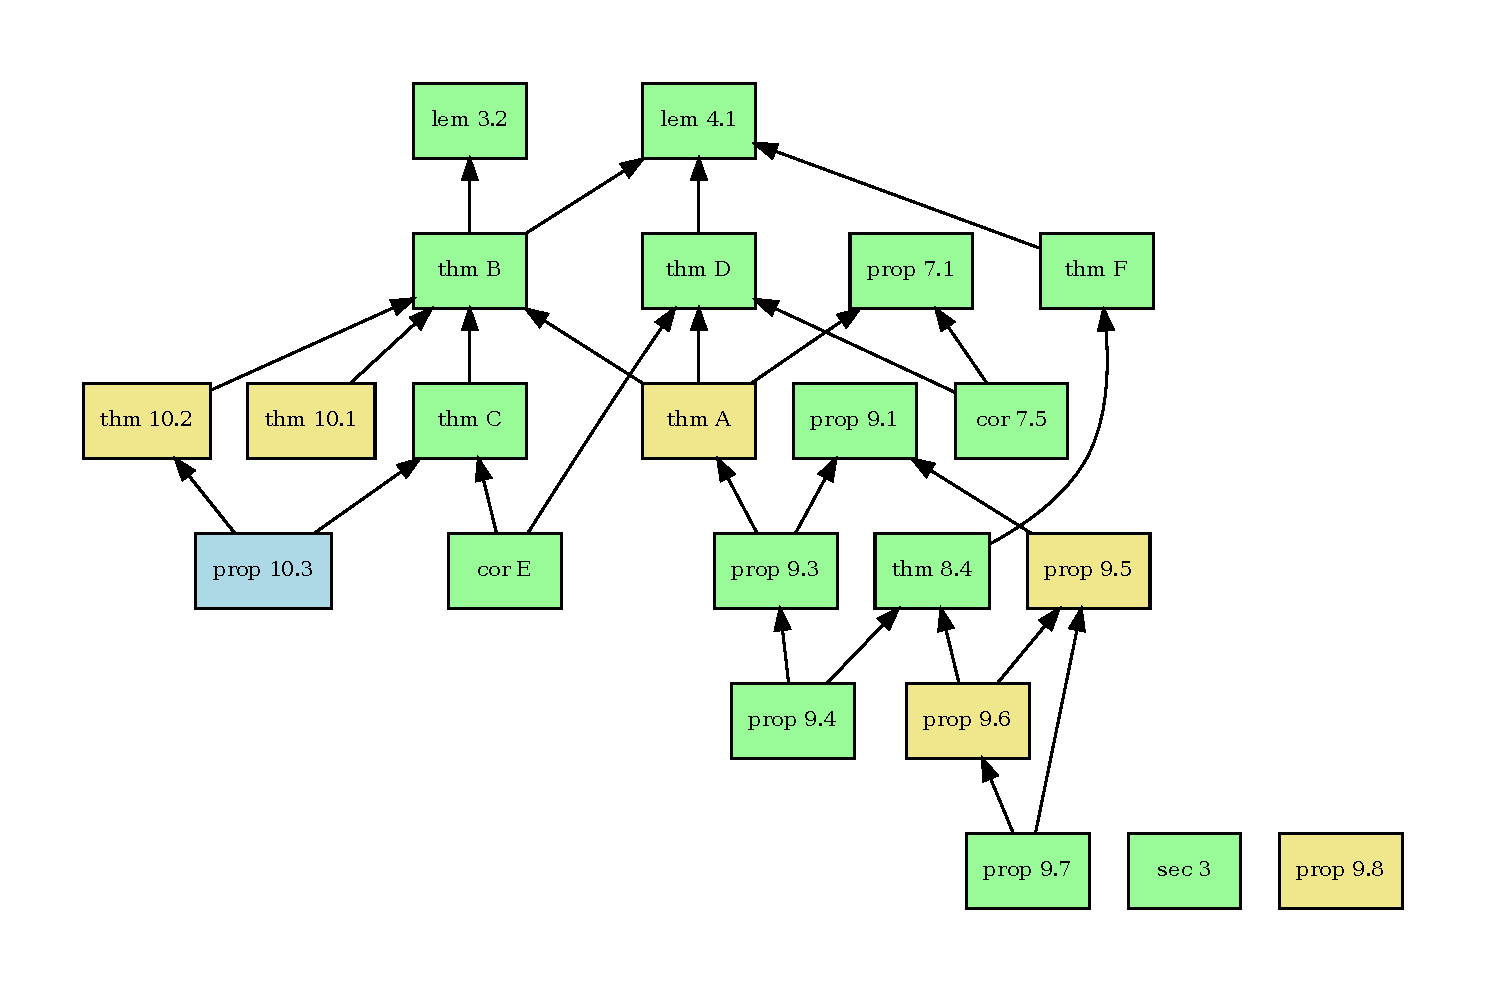
\includegraphics[width=\textwidth,height=0.8\textheight,keepaspectratio]{dep_graph.pdf}\end{center}
\section*{Import graph of the Lean modules}
\begin{center}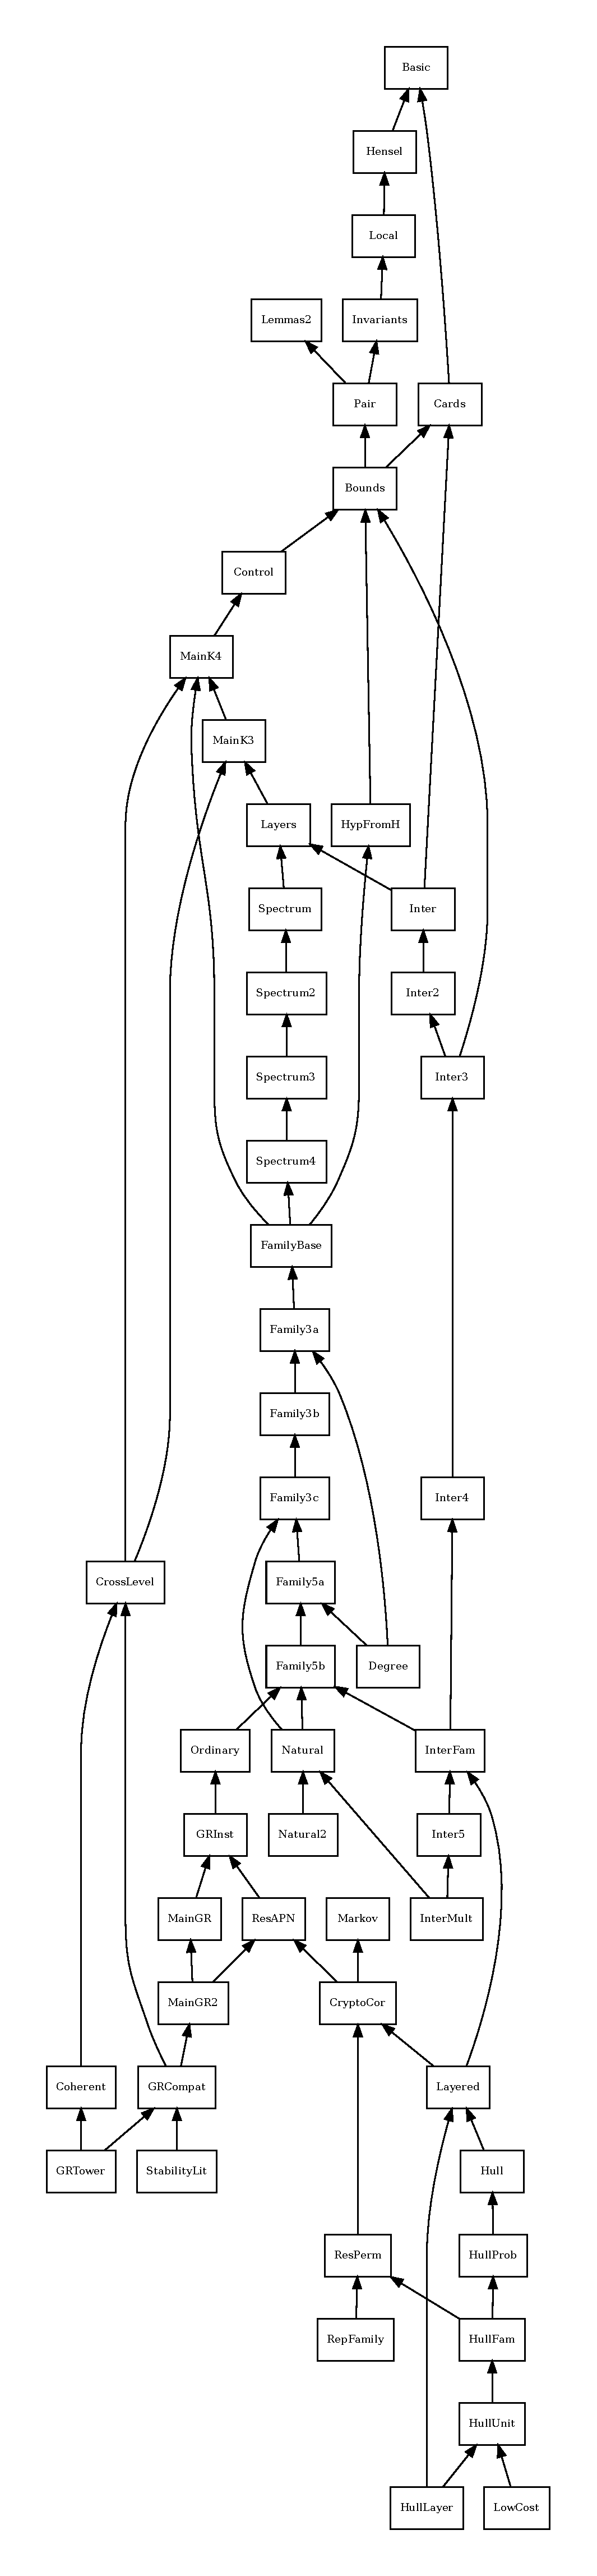
\includegraphics[width=\textwidth,height=0.85\textheight,keepaspectratio]{lean_imports.pdf}\end{center}
\end{document}